\section{OSRKit}

In this section we present a preliminar experimental study of \osrkit. In particular, we aim at addressing the following questions:

\begin{description}[labelindent=1em ,labelsep*=1em,leftmargin=3.5em,itemsep=3pt,parsep=3pt]
\item[Q1] How much does a never-firing OSR point impact code quality? What kind of slowdown should we expect?
\item[Q2] What is the run-time overhead of an OSR transition, for instance to a clone of the running function?
\item[Q3] What is the overhead of \osrkit\ for inserting OSR points and creating a stub or a continuation function?
\end{description}

\missing


\subsection{Experimental Setup}

\subsubsection*{Benchmarks}
We address questions Q1-Q3 by analyzing the performance of \osrkit\ on a selection of the \shootout\ benchmarks, also known as the Computer Language Benchmarks Game~\cite{shootout}, running in \tinyvm. In particular, we focus on single-threaded benchmarks that do not rely on external libraries to perform their core computations. Benchmarks and their description are reported in \mytable\ref{tab:osr-shootout}; four of them ({\tt b-trees}, {\tt mbrot}, {\tt n-body} and {\tt sp-norm}) are evaluated against two workloads of different size.

\begin{table}[ht]
\begin{center}
\begin{small}
    \begin{tabular}{ |c|c| }
        \hline
        Benchmark & Description \\ 
        \hline
        \hline
        b-trees & Adaptation of a GC bench for binary trees \\ 
        \hline
        fannkuch & Fannkuch benchmark on permutations \\ 
        \hline
        fasta & Generation of DNA sequences \\ 
        \hline
        fasta-redux & Generation of DNA sequences (with lookup table) \\ 
        \hline
        mbrot & Mandelbrot set generation \\ 
        \hline
        n-body & N-body simulation of Jovian planets \\ 
        \hline
        rev-comp & Reverse-complement of DNA sequences \\ 
        \hline
        sp-norm & Eigenvalue calculation with power method \\ 
        \hline
    \end{tabular} 
\end{small}
\end{center}
\caption{\label{tab:osr-shootout} Description of the \shootout\ benchmarks.} 
\end{table}

We generate the IR modules for our experiments with \clang\ starting from the C version of the \shootout\ suite. To cover scenarios where OSR machinery is inserted in programs with different optimization levels, we consider two versions: 1) {\em unoptimized}, where the only LLVM optimization we perform is {\tt mem2reg} to promote stack references to registers and construct the SSA form; 2) {\em optimized}, where we apply {\tt opt} {\tt -O1} to the unoptimized version.

\subsubsection*{Environment}
\tinyvm\ supports interactive invocations of functions and it can compile LLVM IR either generated at run-time or loaded from disk. The main design goal behind \tinyvm\ is the creation of an interactive environment for IR manipulation and JIT-compilation of functions: for instance, it allows the user to insert OSR points in loaded functions, run optimization passes on them or display their CFGs, repeatedly invoke a function for a specified amount of times and so on.

\tinyvm\ supports dynamic library loading and linking, and comes with a helper component for MCJIT that simplifies tasks such as handling multiple IR modules, symbol resolution in the presence of multiple versions of a function, and tracking native code and other machine-level generated object such as Stackmaps. \tinyvm\ is thus an ideal playground to exercise our OSR technique.

\subsubsection*{Platform}
Experiments were performed on an octa-core 2.3Ghz Intel Xeon E5-4610 v2 with 256+256KB of L1 cache, 2MB of L2 cache, 16MB of shared L3 cache, and 128 GB of DDR3 main memory, running Debian Wheezy 7, Linux kernel 3.2.0, LLVM 3.6.2 (Release build, compiled using gcc 4.7.2), 64 bit. For each benchmark we analyze CPU time performing 10 trials preceded by an initial warm-up iteration; reported confidence intervals are stated at 95\% confidence level.

\subsection{Impact on Code Quality}

\ifdefined\noauthorea
\begin{figure}[!ht]
\begin{center}
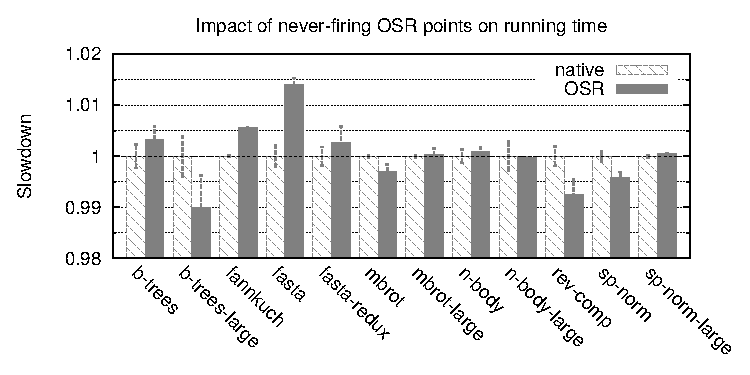
\includegraphics[width=0.65\textwidth]{figures/osr-code-quality-base/osr-code-quality-base.eps}
\caption{\protect\label{fig:osr-code-quality-base} Q1: Impact on running time of never-firing OSR points inserted inside hot code portions (unoptimized code).


}
\end{center}
\end{figure}
\fi

\ifdefined\noauthorea
\begin{figure}[ht]
\begin{center}
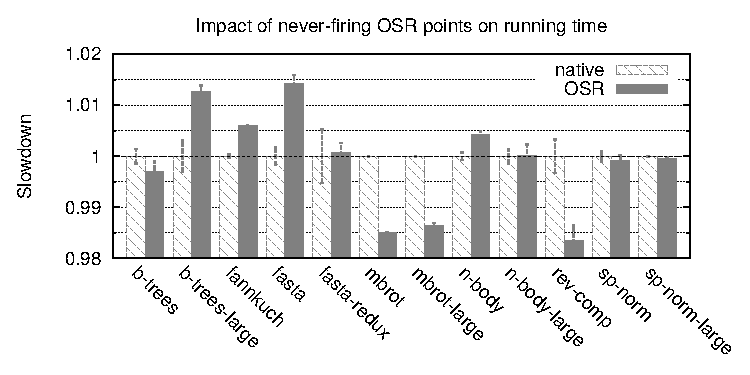
\includegraphics[width=0.65\textwidth]{figures/osr-code-quality-O1/osr-code-quality-O1.eps}
\caption{\protect\label{fig:osr-code-quality-O1} Q1: Impact on running time of never-firing OSR points inserted inside hot code portions (optimized code).



}
\end{center}
\end{figure}
\fi

In order to measure how much a never-firing OSR point might impact code quality (Q1), we analyzed the source-code structure of each benchmark and profiled its run-time behavior to identify performance-critical sections for OSR point insertion. The distinction between open and resolved OSR points is nearly irrelevant in this context: we choose to focus on open OSR points, passing {\tt null} as the {\tt val} argument for the stub (see \missing).

For iterative benchmarks, we insert an OSR point in the body of their hottest loops. We classify a loop as hottest when its body is executed for a very high cumulative number of iterations (e.g., from millions up to billions) and it either calls the method with the highest {\em self} time in the program, or it performs the most computational-intensive operations for the program in its own body.

These loops are natural candidates for OSR point insertion: for instance, the Jikes RVM inserts yield points on backward branches to trigger operations such as method recompilation through OSR and thread preemption for garbage collection. In the \shootout\ benchmarks, the number of such loops is typically 1 (2 for {\tt spectral-norm}).

For recursive benchmarks, we insert an OSR point in the body of the method that accounts for the largest {\em self} execution time in the program. Such an OSR point might be useful to trigger recompilation of the code at a higher degree of optimization, enabling for instance multiple levels of inlining for non-tail-recursive functions. The only analyzed benchmark showing a recursive pattern is {\tt b-trees}.

Results for the unoptimized and optimized versions of the benchmarks are reported in \myfigure\ref{fig:osr-code-quality-base} and \myfigure\ref{fig:osr-code-quality-O1}, respectively. For both scenarios we observe that the overhead is very small, i.e., less than $1\%$ for most benchmarks and less than $2\%$ in the worst case. For some benchmarks, code might run slightly faster after OSR point insertion due to instruction cache effects.
%We analyzed the code produced by the x86-64 back-end: the OSR machinery is lowered into three native instructions that load a counter in a register, compare it against a constant value and jump to the OSR block accordingly.
The number of times the OSR condition is checked for each benchmark is 
%the same as in the experiments 
reported in \mytable\ref{tab:osr-sameFun}.

\subsection{Overhead of OSR Transitions}

\mytable\ref{tab:osr-sameFun} reports estimates of the average cost of performing an OSR transition to a clone of the running function (Q2). For each benchmark we compute the time difference between the scenarios in which an always-firing and a never-firing resolved OSR point is inserted in the code, respectively; we then normalize this difference against the number of fired OSR transitions.

\begin{table}[ht]
\begin{center}
\begin{small}
% hack for wrapping: http://tex.stackexchange.com/questions/54069/table-with-text-wrapping
\newcolumntype{A}{>{\centering\arraybackslash}m{1.33cm}}
\newcolumntype{B}{>{\centering\arraybackslash}m{1.00cm}}
\newcolumntype{C}{>{\centering\arraybackslash}m{1.15cm}}
    \begin{tabular}{ |c|A|B|C|B|C| }
        \cline{3-6}
        \multicolumn{2}{c|}{} & \multicolumn{2}{c|}{{\em Unoptimized code}} & \multicolumn{2}{c|}{{\em Optimized code}} \\
        \hline
        Benchmark & Fired OSRs (M) & Live values & Avg time (ns) & Live values & Avg time (ns) \\ 
        \hline
        \hline
        b-trees & 605 & 2 & 1.731 & 3 & 0.974 \\ 
        \hline
        b-trees-large & 2\,690 & 2 & 1.749 & 3 & 1.423 \\ 
        \hline
        fannkuch & 399 & 0 & 1.793 & 0 & 0.621 \\ 
        \hline
        fasta & 400 & 2 & 2.335 & 2 & 2.699 \\ 
        \hline
        fasta-redux & 400 & 4 & 2.306 & 4 & 2.269 \\ 
        \hline
        mbrot & 256 & 15 & 5.016 & 15 & 3.628 \\ 
        \hline
        mbrot-large & 1\,024 & 15 & 5.268 & 15 & 4.637 \\ 
        \hline
        n-body & 50 & 3 & 2.952 & 3 & 6.929 \\ 
        \hline
        n-body-large & 500 & 3 & 2.953 & 3 & 6.953 \\ 
        \hline
        rev-comp & 6 & 8 & -10.158 & 8 & 8.267 \\ 
        \hline
        sp-norm & 1\,210 & 2 & 0.772 & 2 & -0.030 \\ 
        \hline 
        sp-norm-large & 19\,360 & 2 & 0.778 & 2 & -0.003 \\
        \hline
    \end{tabular} 
\end{small}
\end{center}
\caption{\label{tab:osr-sameFun}Cost of OSR transitions to the same function. For each benchmark we report the number of fired OSR transitions (rounded to millions), the number of live values passed at the OSR point, and the average time for a transition.
}
\end{table}

Hot code portions for OSR point insertion have been identified as in the Q1 experiments for code quality. Depending on the characteristics of the hot loop, we either transform its body into a separate function and instrument its entrypoint, or, when the loop calls a method with a high self time, we insert an OSR point at the beginning of that method.

Normalized differences reported in the table represent a reasonable estimate of the average cost of firing an OSR transition.
%, which in other words is the cost of performing a function call passing the live variables as arguments. 
Reported numbers are in the order of nanoseconds, and might be negative due to instruction cache effects. We remark that for this experiment slicing the loop body is preferable to inserting an OSR point in it, as the continuation function should fire an OSR itself at the very next loop iteration and so on, possibly leading to an undesired stack growth.

\subsection{OSR Machinery Generation}

We now discuss the overhead of the \osrkit\ library for inserting OSR machinery in the IR of a function (Q3). \mytable\ref{tab:osr-instrTime} reports for each benchmark the number of IR instructions in the instrumented function and the time spent in the IR manipulation. Locations for OSR points are chosen as in the Q1 experiments, and the target function is a clone of the source function.

\begin{table}[ht]
\begin{small}
    \begin{tabular}{ |c|c|c|c|c|c|c| }
        \cline{3-7}
        \multicolumn{2}{l|}{} & \multicolumn{2}{c|}{{\em Open OSR {\tiny$(\mu s)$}}} & \multicolumn{3}{c|}{{\em Resolved OSR  {\tiny$(\mu s)$}}} \\ 
        \cline{3-7}
        \multicolumn{2}{l|}{} & Insert & Gen. & Insert & \multicolumn{2}{|c|}{Generate \fosrto} \\ 
        \cline{1-2} \cline{6-7}
        Benchmark & \textbar IR\textbar & point & stub & point & Total & Avg/inst \\
        \hline
        \hline
        b-trees & 13 & 15.40 & 28.32 & 14.31 & 76.13 & 5.86 \\
        \hline
        fannkuch & 50 & 14.16 & 18.66 & 12.84 & 208.03 & 4.16 \\
        \hline
        fasta & 38 & 12.93 & 27.07 & 13.01 & 250.39 & 6.59 \\
        \hline
        fasta-redux & 55 & 13.79 & 23.44 & 9.32 & 258.36 & 4.70 \\
        \hline
        mbrot & 77 & 15.96 & 27.39 & 15.30 & 384.61 & 4.99 \\
        \hline
        n-body & 19 & 14.31 & 19.73 & 11.58 & 88.73 & 4.67  \\
        \hline
        rev-comp & 145 & 16.31 & 39.99 & 13.90 & 810.84 & 5.59 \\
        \hline
        sp-norm & 28 & 15.31 & 27.50 & 12.41 & 154.54 & 5.52 \\ 
        \hline
    \end{tabular} 
\caption{\label{tab:osr-instrTime} Q3: OSR machinery insertion in optimized code. Time measurements are expressed in microseconds. Results for unoptimized code are very similar and thus not reported.}
\end{small}
\end{table}

For open OSR points, we report the time spent in inserting the OSR point in the function and in generating the stub; both operations do not depend on the size of the function. For resolved OSR points, we report the time spent in inserting the OSR point and in generating the \fosrto\ function.

Not surprisingly, constructing a continuation function takes longer than the other operations (i.e., up to 1 ms vs. 20-40 us), as it involves cloning and manipulating the body of the target function and thus depends on its size: \mytable\ref{tab:osr-instrTime} hence comes with an additional column in which time is normalized against the number of IR instructions in the target function.

\subsection{Discussion}
Experimental results presented in the previous sections suggest that inserting an OSR point is unlikely to degrade the quality of generated code (Q1). The time required to fire an OSR transition is negligible (i.e., order of nanoseconds, Q2), while the cost of OSR-point insertion and of generating a continuation function - either when inserting a resolved OSR point, or from the callback method invoked at an open OSR transition - 
is likely to be dominated by the cost of its compilation (Q3).

For a front-end, the choice whether to insert an OSR point into a function for dynamic optimization merely depends on the trade-off between the expected benefits in terms of execution time and the overheads from generating on optimized version of the function and eventually JIT-compiling it; compared to these two operations, the cost of OSR-related operations is negligible. \missing